\begin{frame}\frametitle{Задачи}
    \begin{itemize}
        \item Обеспечить загрузку входных данных
        \item Визуализировать результаты поиска объекта
        \item Склеить написанный код в единый проект
    \end{itemize}
\end{frame}

\begin{frame}\frametitle{Технологии}
    \begin{itemize}
        \item PySide (Qt) - GUI
        \item OpenGL      - Отрисовка модели объекта на ключевом кадре
    \end{itemize}
\end{frame}

\begin{frame}\frametitle{Процесс разработки}
    Написаны:
    \begin{itemize}
        \item модуль для загрузки ключевых кадров
        \item CLI-интерфейс для работы с ними
        \item рендер объекта при помощи OpenGL
        \item GUI-интерфейс для удобства работы
    \end{itemize}
\end{frame}

\begin{frame}\frametitle{GUI}
    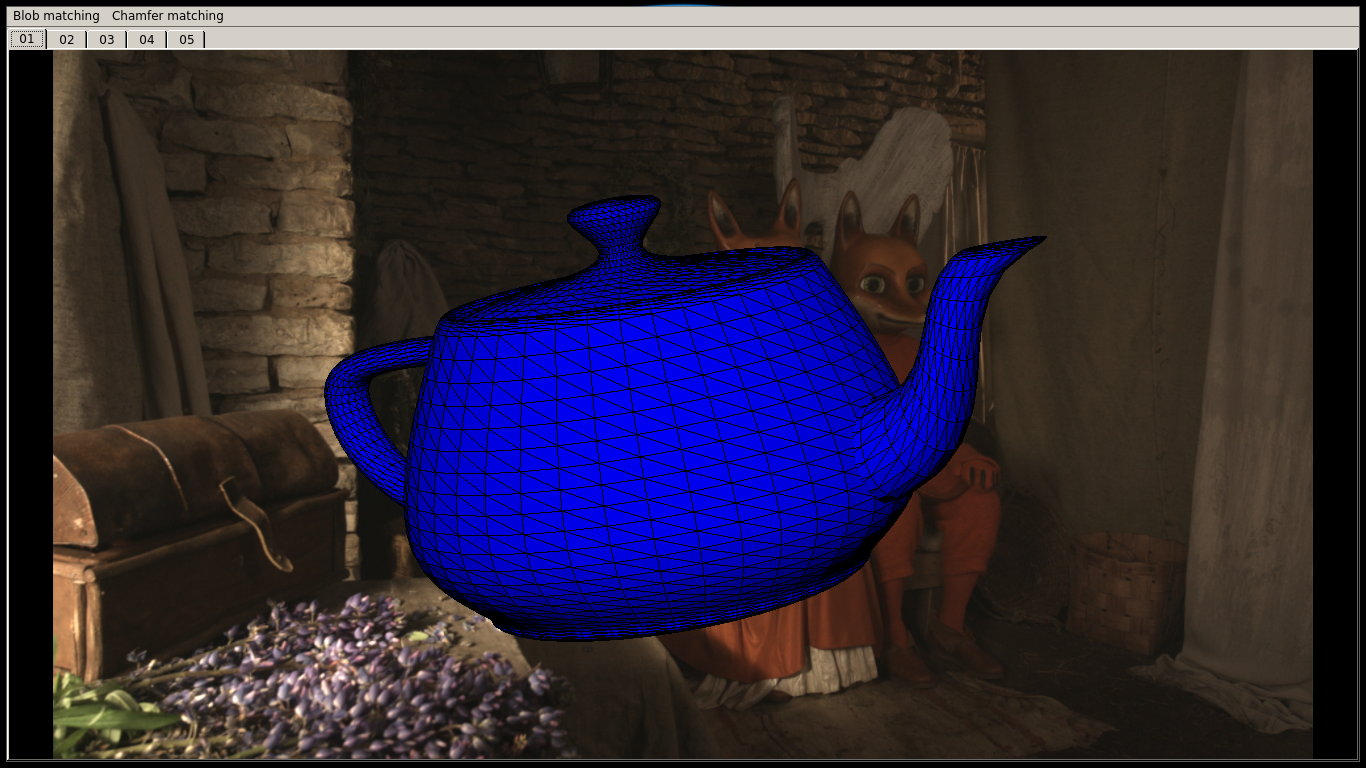
\includegraphics[height=6cm]{gui_samples/sample_01.png}
\end{frame}

\begin{frame}\frametitle{GUI}
    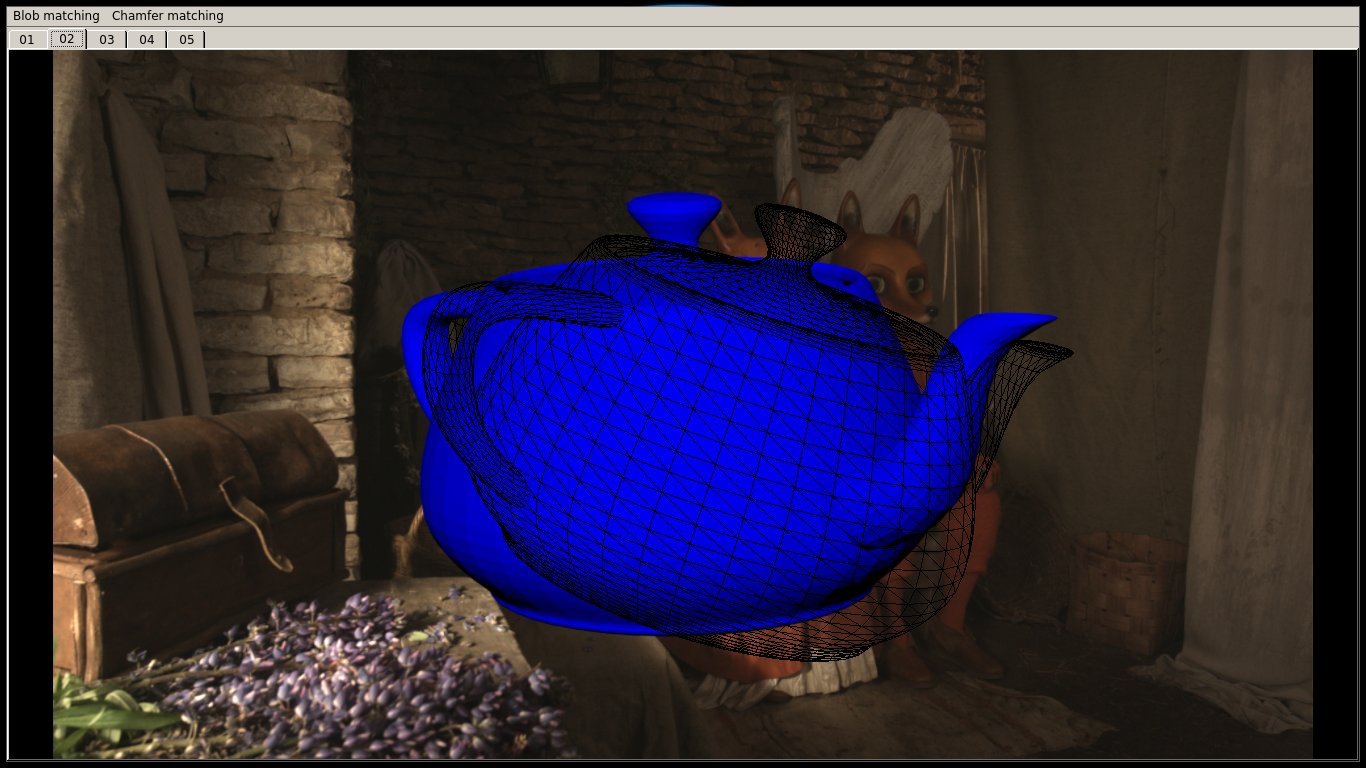
\includegraphics[height=6cm]{gui_samples/sample_02.png}
\end{frame}

\begin{frame}\frametitle{Результаты}
    \begin{itemize}
        \item Получился относительно цельный проект
        \item Все работает и шуршит
        \item Я разобрался с OpenGL и его использованием в Qt
    \end{itemize}
\end{frame}
